% Options for packages loaded elsewhere
\PassOptionsToPackage{unicode}{hyperref}
\PassOptionsToPackage{hyphens}{url}
\documentclass[
]{article}
\usepackage{xcolor}
\usepackage[margin=1in]{geometry}
\usepackage{amsmath,amssymb}
\setcounter{secnumdepth}{5}
\usepackage{iftex}
\ifPDFTeX
  \usepackage[T1]{fontenc}
  \usepackage[utf8]{inputenc}
  \usepackage{textcomp} % provide euro and other symbols
\else % if luatex or xetex
  \usepackage{unicode-math} % this also loads fontspec
  \defaultfontfeatures{Scale=MatchLowercase}
  \defaultfontfeatures[\rmfamily]{Ligatures=TeX,Scale=1}
\fi
\usepackage{lmodern}
\ifPDFTeX\else
  % xetex/luatex font selection
\fi
% Use upquote if available, for straight quotes in verbatim environments
\IfFileExists{upquote.sty}{\usepackage{upquote}}{}
\IfFileExists{microtype.sty}{% use microtype if available
  \usepackage[]{microtype}
  \UseMicrotypeSet[protrusion]{basicmath} % disable protrusion for tt fonts
}{}
\makeatletter
\@ifundefined{KOMAClassName}{% if non-KOMA class
  \IfFileExists{parskip.sty}{%
    \usepackage{parskip}
  }{% else
    \setlength{\parindent}{0pt}
    \setlength{\parskip}{6pt plus 2pt minus 1pt}}
}{% if KOMA class
  \KOMAoptions{parskip=half}}
\makeatother
\usepackage{graphicx}
\makeatletter
\newsavebox\pandoc@box
\newcommand*\pandocbounded[1]{% scales image to fit in text height/width
  \sbox\pandoc@box{#1}%
  \Gscale@div\@tempa{\textheight}{\dimexpr\ht\pandoc@box+\dp\pandoc@box\relax}%
  \Gscale@div\@tempb{\linewidth}{\wd\pandoc@box}%
  \ifdim\@tempb\p@<\@tempa\p@\let\@tempa\@tempb\fi% select the smaller of both
  \ifdim\@tempa\p@<\p@\scalebox{\@tempa}{\usebox\pandoc@box}%
  \else\usebox{\pandoc@box}%
  \fi%
}
% Set default figure placement to htbp
\def\fps@figure{htbp}
\makeatother
\setlength{\emergencystretch}{3em} % prevent overfull lines
\providecommand{\tightlist}{%
  \setlength{\itemsep}{0pt}\setlength{\parskip}{0pt}}
\usepackage[]{natbib}
\bibliographystyle{plainnat}
\usepackage{booktabs}
\usepackage{longtable}
\usepackage{array}
\usepackage{multirow}
\usepackage{wrapfig}
\usepackage{float}
\usepackage{colortbl}
\usepackage{pdflscape}
\usepackage{tabu}
\usepackage{threeparttable}
\usepackage{threeparttablex}
\usepackage[normalem]{ulem}
\usepackage{makecell}
\usepackage{xcolor}
\usepackage{bookmark}
\IfFileExists{xurl.sty}{\usepackage{xurl}}{} % add URL line breaks if available
\urlstyle{same}
\hypersetup{
  pdftitle={A natural account of loss aversion},
  hidelinks,
  pdfcreator={LaTeX via pandoc}}

\title{A natural account of loss aversion}
\author{Ansgar D. Endress \& Peter Ayton}
\date{}

\begin{document}
\maketitle

\subsection{Basic idea}\label{basic-idea}

The current model also provides a natural explanation of loss aversion
in prospect theory. In a nutshell, the absolute subjective value (i.e.,
the utility) of a change in endowment is greater for losses than for
gains - according to some meta-analyses about 1.995 times as large
\citep{Brown2024} (but see below). While this observation has been
considered ``the most significant contribution of psychology to
behavioral economics'' (\citep{Kahneman2011}, p.~300), it is usually
treated as a quirk of human decision making by fitting arbitrary
parameters to human performance
\citep{Tversky1992, Abdellaoui2007, Booij2009}.

Instead, we propose that loss aversion is an automatic consequence of
our biophysically-rooted decision model. Specifically, we propose that,
with respect to an endowment \(E\), the subjective desirability (i.e.,
the utility) of a positive change \(C\) tracks the subjective certainty
that the change is a gain, which, in turn tracks the Weber ratio
\(\frac{E + C}{E}\). Conversely, the subjective \emph{undesirability} of
a negative change (i.e., the utility) tracks the subjective certainty
that the change is a loss, which, in turn, tracks the Weber ratio
\(\frac{E}{E + C}\) (for negative \(C's\)).

The Weber ratio for losses \(\frac{E}{E - |C|}\) is strictly greater
than that for gains \(\frac{E + |C|}{E}\), where \(|C|\) is the absolute
value of \(C\).\footnote{Proof: Assume that
  \(\frac{E}{E - |C|} < \frac{E + |C|}{E}\). It follows that
  \(E^2 < (E + |C|)(E - |C|)\), and thus that \(|C|^2 < 0\), which is a
  contradiction.} Since the acceptability function is monotonic, the
absolute utility of losses is thus strictly greater than that of gains.
In other words, loss aversion is a basic consequence of magnitude
processing, and thus of any system with a fixed precision and
multiplicative gain control \citep{Endress-Catastrophic-Interference}.

\begin{figure}

{\centering 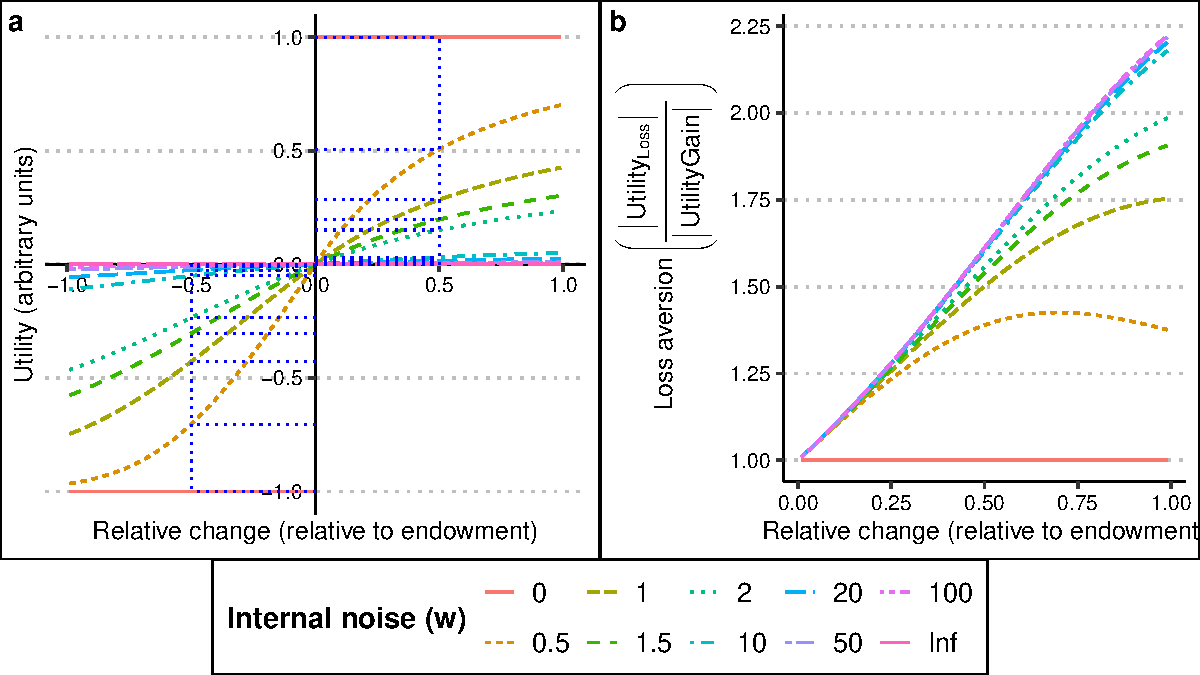
\includegraphics[width=0.8\linewidth]{loss_aversion_files/figure-latex/loss-aversion-demo-plot-1} 

}

\caption{Illustration of loss aversion as a consequence of magnitude processing. (a) Subjective utility as a function of relative gains or losses with respect to an endowment, for different values of the uncertainty parameter $w$. The S-shaped curve emerges naturally from the asymmetry of the Weber ratios for gains and losses. Dotted blue lines mark the utility values at a change of $\pm 50\%$, illustrating that the absolute utility of a $50\%$ loss exceeds that of a $50\%$ gain. (b) Ratio of absolute utilities for losses vs.\ gains, $\frac{\left|\text{Utility}_{\text{Loss}}\right|}{\left|\text{Utility}_{\text{Gain}}\right|}$, as a function of relative change. Values greater than 1 indicate loss aversion. Note that loss aversion exceeds 1 for all values of $w$ and increases with the size of the change.}\label{fig:loss-aversion-demo-plot}
\end{figure}

This idea is illustrated in Figure \ref{fig:loss-aversion-demo-plot}.
Figure \ref{fig:loss-aversion-demo-plot}a plots the subjective value as
a function of relative changes with respect to the endowment between
-99\% and 99\%, and shows the typical S-shaped curve. Figure
\ref{fig:loss-aversion-demo-plot}b plots the relative utility for loss
vs.~gains for a given change,
i.e.~\(\frac{\left|\text{Utility}_{\text{Loss}}\right|}{\left|\text{Utility}_{\text{Gain}}\right|}\).
The relative utility is a measure of loss aversion. For example, if
\(\frac{\left|\text{Utility}_{\text{Loss}}\right|}{\left|\text{Utility}_{\text{Gain}}\right|} = 2\)
for a given change, the change is twice as aversive as a loss as it
would be positive as a gain. Figure \ref{fig:loss-aversion-demo-plot}b
shows that the relative utility is always greater than 1, and thus shows
loss aversion for all uncertainty parameters \(w\). Further, we make the
novel prediction that the relative utility of losses (compared to gains)
should increase as a function of change (see below), a prediction that
receives support from different studies
\citep{Abdellaoui2007, Booij2009}.

\subsection{\texorpdfstring{Comparison to
\citep{Tversky1992}}{Comparison to {[}@Tversky1992{]}}}\label{comparison-to-tversky1992}

\begin{figure}

{\centering 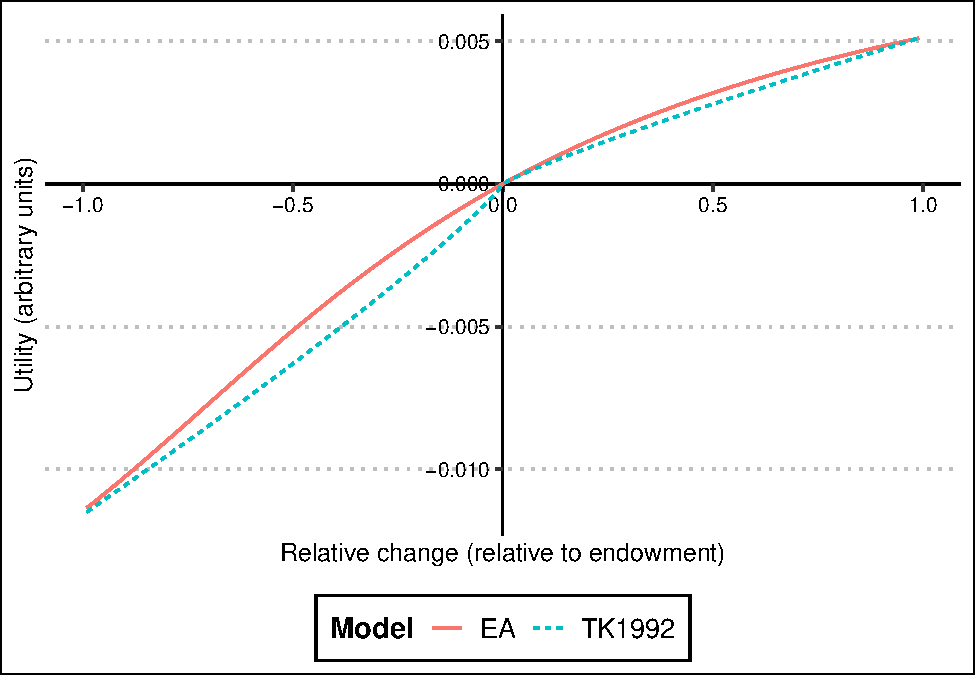
\includegraphics[width=0.8\linewidth]{loss_aversion_files/figure-latex/tk-plot-1} 

}

\caption{Comparison of the current model (EA) and the Tversky and Kahneman (1992) model, with parameterization $\lambda = 2.25$, $\alpha = \beta = 0.88$. The $w$ parameter was set to a large value ($w = 10$) to approximate the quasi-linear behavior of the Tversky and Kahneman (1992) function. Because both models use arbitrary units, the output of the Tversky and Kahneman (1992) model was scaled so that the maxima of both functions coincide. The two models produce closely overlapping value functions across the full range of relative changes.}\label{fig:tk-plot}
\end{figure}

In Figure \ref{fig:tk-plot}, we show that our model can mimic the
functional form assumed by \citep{Tversky1992}. We use their
parameterization (\(\text{utility} = |C|^\alpha - \lambda |C|^\beta\),
with \(\lambda = 2.25\) and \(\alpha = \beta = 0.88\), but see below).
We thus set the \(w\) parameter to a large value to make it quasi-linear
as in their function (\(w = 10\)). Given that both models use arbitrary
units, we multiplied the output of the Tversky and Kahneman model so
that the maximum y value coincide for both models. As shown in Figure
\ref{fig:tk-plot}, both models behave fairly similarly.

\subsection{\texorpdfstring{Variability of \(\lambda\)
estimates}{Variability of \textbackslash lambda estimates}}\label{variability-of-lambda-estimates}

While \citep{Tversky1992} proposed a \(\lambda\) value of 2.25, there is
considerable variability across studies, with some metanalyses finding a
value of 1.995 \citep{Brown2024}, others of 1.31 \citep{Walasek2024} and
yet others of 1.07 \citep{Yechiam2025}. Further, methodological
differences seems to affect the magnitude of loss aversion, including
how the parameter is estimated, the population \citep{Brown2024}, and
the size of the magnitude of the gain/loss
\citep{Abdellaoui2007, Booij2009}, with some authors even proposing that
loss aversion mainly arises in experiments where gains are larger than
losses and where gains and losses are presented in an ordered fashion
\citep{Yechiam2025}.

While our simple conceptual model is not intended to capture such
variability, variability is expected for a variety of reasons. For
example, and as mentioned above, we predict that loss aversion depends
on the relative change. Likewise, given that number processing shows
substantial individual differences in the \(w\) parameter
\citep{Halberda2008}, we would expect similar individual differences in
loss aversion. To the extent that observers retain numeric information
over trials, we would also expect to see ordering effects like those in
\citep{Yechiam2025}, for example through anchoring effects across
trials. However, further research is needed to map our model to such
differences in loss aversion.

\subsection{Integration of probabilistic
information}\label{integration-of-probabilistic-information}

In standard prospect theory, utilities are integrated with probability
information. However, given that humans use approximate representations
of numbers even when these numbers are presented as Arabic numerals
\citep{Moyer1967, Buckley1974, Hinrichs1981, Dehaene1990}, the
assumption that probalistic information is represented at face value is
almost certainly false (see also \citep{BarrettoGarcia2023, Khaw2020}
for evidence that risk taking is related to number processing
precision). As a result, to construct a biophysically grounded
derivation of prospect theory, more work is need to understand how
probabilistic information is represented, and how the (presumably) noisy
representations of probability information is integrated with the noisy
representations of value.

\subsection{Monotonicity behavior {[}We will probably remove this
section eventually, but I keep it in case I have a better idea for the
proof{]}}\label{monotonicity-behavior-we-will-probably-remove-this-section-eventually-but-i-keep-it-in-case-i-have-a-better-idea-for-the-proof}

In this section, we investigate whether the relative utility of losses
vs.~gains is growing. With the acceptability given by
\(1 + \log_2 \Phi\left(\frac{R-1}{\sqrt{2}w \sqrt(R^2 + 1)}\right)\), we
get

\[
G(C) =  \frac{1 + \log_2 \Phi \left( \frac{\frac{E}{E-C} - 1}{\sqrt{2}w \sqrt{\left(\frac{E}{E-C}\right)^2 + 1}} \right)}{1 + \log_2 \Phi \left( \frac{\frac{E+C}{E} - 1}{\sqrt{2}w \sqrt{\left(\frac{E+C}{E}\right)^2 + 1}} \right)} = \frac{1 + \log_2 \Phi \left( \frac{C}{\sqrt{2}w \sqrt{E^2 + (E-C)^2}} \right)}{1 + \log_2 \Phi \left( \frac{C}{\sqrt{2}w \sqrt{(E+C)^2 + E^2}} \right)}
\]

where we assume that \(C\) is non-negative. While the derivative is
cumbersome to calculate, is easy to see that \(G(C) > 1\) for all
\(C's\) between \(0\) and \(E\), and that \(G(C)\) must be locally
growing for at least some \(C\) in the neighborhood of \(0\).

In fact, for \(C = 0\), L'Hôpital's Rule shows that \(G(C)\) converges
to \(1\). For all \(0 < C < E\), the Weber ratio in the numerator is
strictly greater than that in the denominator. As both \(log_2\) and
\(\Phi\) are strictly monotonic, \(G(C)\) is greater than \(1\) for all
\(0 < C < E\).

As a result, the Mean Value Theorem implies that, for each
\(0 < C < E\), there exists an \(C^*\) for which \(G^\prime(C^*)\) is
strictly positive. While this does not imply that \(G\) grows
monotonically, it does imply that the one can find \(C^*\)'s where
\(G^\prime\) is positive in arbitrarily small neighborhoods of \(0\),
and that the average growth around \(C = 0\) is positive.

To avoid differentiating an unwieldy function, we consider the
difference in utilities.

\[
H(C) =  1 + \log_2 \Phi \left( \frac{\frac{E}{E-C} - 1}{\sqrt{2}w \sqrt{\left(\frac{E}{E-C}\right)^2 + 1}} \right) - \left(1 + \log_2 \Phi \left( \frac{\frac{E+C}{E} - 1}{\sqrt{2}w \sqrt{\left(\frac{E+C}{E}\right)^2 + 1}} \right)\right) = \log_2 \Phi \left( \frac{C}{\sqrt{2}w \sqrt{E^2 + (E-C)^2}} \right) -  \log_2 \Phi \left( \frac{C}{\sqrt{2}w \sqrt{(E+C)^2 + E^2}} \right)
\]

\bibliography{/Users/endress/ansgar.bib}

\end{document}
